\documentclass{standalone}
\usepackage{tikz}
\usepackage{ctex,siunitx}
\setCJKmainfont{Noto Serif CJK SC}
\usepackage{tkz-euclide}
\usepackage{amsmath}
\usetikzlibrary{patterns, calc,3d}
\usetikzlibrary {decorations.pathmorphing,decorations.pathreplacing,decorations.shapes}
\tikzset{label style/.append style={font=\small}}
\begin{document}
\small
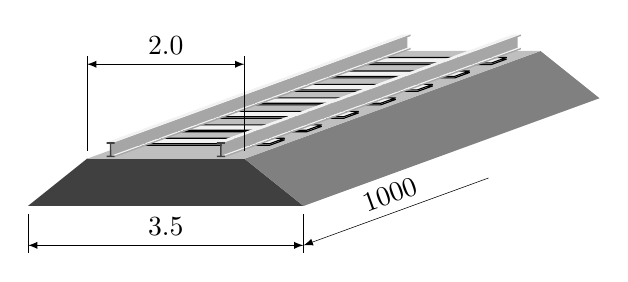
\begin{tikzpicture}[>=latex,scale=1.0]
  \tkzDefPoints{-1.75/0/A,1.75/0/B,1/0.6/C,-1/0.6/D}
  \tkzDrawPolygon[draw=none,fill=darkgray](A,B,C,D)
  \foreach \x in {B,C,D}
  {\tkzDefShiftPoint[\x](20:4){\x'}}
  \tkzDrawPolygon[draw=none,fill=gray](B,B',C',C)
  \tkzDrawPolygon[draw=none,fill=lightgray](D,D',C',C)
  \foreach \r in {1,...,7}
  {
    \draw[line join=round]([shift=(20:0.5*\r)]0,0.6)--++(0.85,0)--++(20:0.2)--++(-1.7,0)--++(20:-0.2)--cycle;
    \draw[fill=lightgray!20,line join=round]([shift=(20:0.5*\r)]0,0.62)--++(0.85,0)--++(20:0.2)--++(-1.7,0)--++(20:-0.2)--cycle;
  }
  
  \foreach \x in {-0.7,0.7}
  {
    \fill[gray!70](\x+0.01,0.64)--++(20:4)--++(0,0.15)--++(20:-4)--cycle;
    \fill[gray!70](\x+0.05,0.62)--++(20:4)--++(0,0.02)--++(20:-4)--cycle;
    \fill[gray!70](\x+0.05,0.79)--++(20:4)--++(0,0.02)--++(20:-4)--cycle;
    \fill[lightgray!20](\x+0.05,0.81)--++(20:4)--++(-0.1,0)--++(20:-4)--cycle;
    \fill[lightgray!20](\x+0.05,0.64)--++(20:4)--++(-0.04,0)--++(20:-4)--cycle;
    \fill[darkgray](\x-0.05,0.62)--++(0.1,0)--++(0,0.02)--++(-0.04,0)--++(0,0.15)--++(0.04,0)--++(0,0.02)--++(-0.1,0)--++(0,-0.02)--++(0.04,0)--++(0,-0.15)--++(-0.04,0)--cycle;
  }

  \draw[very thin](-1,0.7)--++(0,1.2)(1,0.7)--++(0,1.2);
  \draw[very thin,<->](-1,1.8)--(1,1.8)node[midway,above]{2.0};
  \draw[very thin](-1.75,-0.1)--(-1.75,-0.6)(1.75,-0.1)--(1.75,-0.6);
  \draw[very thin,<->](-1.75,-0.5)--(1.75,-0.5)node[midway,above]{3.5};
  \draw[very thin,<-](1.75,-0.5)--++(20:2.5)node[midway,sloped,above]{1000};
\end{tikzpicture}
\end{document}